\question 假设某计算机按字编址,Cache有4个行,Cache和主存之间交换的块大小为1个字。若Cache的内容初始为空,采用2路组相联映射方式和LRU替换算法,当访问的主存地址依次为0,4,8,2,0,6,8,6,4,8时,命中Cache的次数是(
)
\par\twoch{1}{2}{\textcolor{red}{3}}{4}
\begin{solution}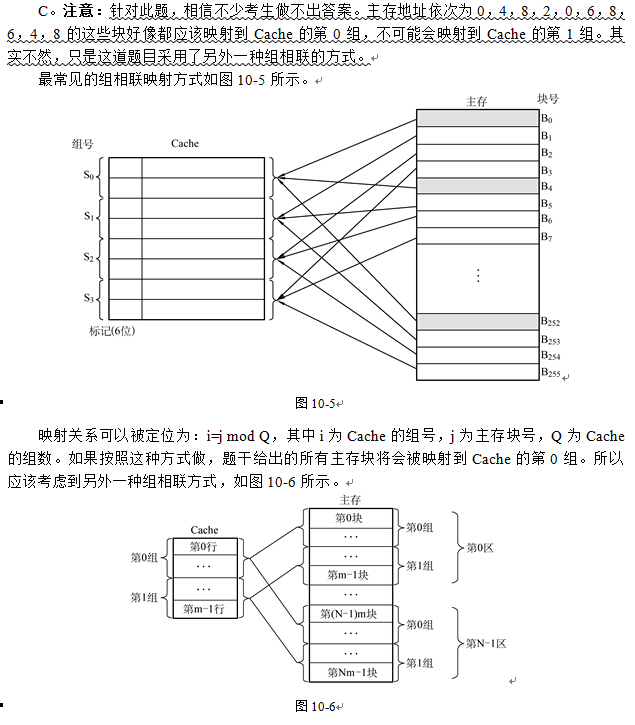
\includegraphics[width=6.61458in,height=7.55208in]{computerassets/ff0c95e262008e1450dfd6e70ac0cf03.jpeg}
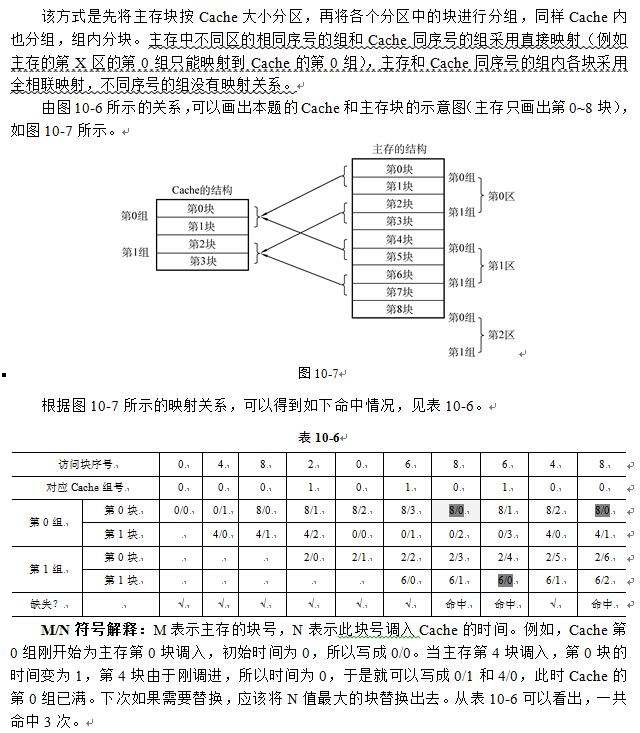
\includegraphics[width=6.66667in,height=7.63542in]{computerassets/3f06ac0859d8a5c827fb5e5c108f981b.jpeg}
\end{solution}
